%   % !TEX root = ../../VIII,3_Rahmen-TeX_8-1.tex
%
%
%   Band VIII, 3 N.~??A26
%   Signatur/Tex-Datei: LH_35_14_02_047
%   RK-Nr. 58242
%   Überschrift: [Ratio tensionis et longitudinis in chordis (ex: Sit funis F)]
%   Modul: Mechanik // AEF (Elastizität, Akustik)
%   Datierung: [Ende Dezember 1689 bis Frühjahr 1690 (?)]
%   WZ: 803012 = RK-WZ 409 = Kreuz auf drei Kreisen/Ringen in senkr. Reihe, darunter cBv / GBV?
%   SZ: keins
%   Bilddateien (PDF): LH_35_14_02_047_d1; LH_35_14_02_047_d2; LH_35_14_02_047_d3 (insgesamt: drei)
%   e Storckio
%
%
\selectlanguage{ngerman}%
\frenchspacing%
%
\begin{ledgroupsized}[r]{120mm}%
\footnotesize%
\pstart%
\noindent%
\textbf{Überlieferung:}%
\pend%
\end{ledgroupsized}%
\begin{ledgroupsized}[r]{114mm}%
\footnotesize%
\pstart%
\parindent -6mm%
\makebox[6mm][l]{\textit{L}}%
Aufzeichnung: LH~XXXV~14,~2 Bl.~47.
Ein Zettel (10,7 x 10,1 cm),
ursprünglich mit LH~XXXV~14,~2 Bl.~46 zusammenhängend; % RK 58241
Fragment eines Wasserzeichens: italienisches Papier.
Zwei Seiten;
Bl.~47~v\textsuperscript{o} überliefert ferner die Diagramme \lbrack\textit{Fig.~2}\rbrack\ und \lbrack\textit{Fig.~3}\rbrack\ von N.~30.
\pend%
\end{ledgroupsized}%
%
\vspace*{5mm}%
\begin{ledgroup}%
\footnotesize%
\pstart%
\noindent%
\textbf{Datierungsgründe:}\label{LH_35_14_02_047_datierung}
Der Träger der vorliegenden Aufzeichnung hing ursprünglich mit LH~XXXV~14,~2 Bl.~46 zusammen, einem Bogen, der einen Teil von N.~30 sowie einen noch in \textit{LSB} VIII zu edierenden Auszug aus Galileis \textit{Discorsi} überliefert.%
\protect\index{Namensregister}{\textso{Galilei} (Galilaeus, Galileus), Galileo 1564\textendash1642}
Auf Bl.~46 findet sich dasselbe Wasserzeichen wie auf weiterem Papier, das Leibniz während seines Aufenthalts in der italienischen Stadt Modena von Ende Dezember 1689 bis Anfang Februar 1690 (\textit{Chronik}, S.~99–101\cite{01236}) verwendete, etwa bei den ersten Fassungen des Textes N.~31 (siehe die Datierungsgründe, S.~\pageref{LH_35_10_17_005-008_intro}).%
\protect\index{Ortsregister}{Modena}\protect\index{Ortsregister}{Italien}
Wie im Fall von N.~31 könnten Gespräche mit dem dortigen Mathematiker G.\,B. Boccabadati die in N.~29 überlieferten Ausführungen über das Verhältnis zwischen Spannkraft und Dehnung einer Saite bzw. eines Seils veranlasst haben.\protect\index{Namensregister}{\textso{Boccabadati} (Boccabadatus), Giovan Battista 1635\textendash1696}
Leibniz könnte aber auch nach seiner Abreise aus Modena den Zettel abgeschnitten und N.~29 verfasst haben.
Die Verwendung des genannten Papiers im Leibniz-Nachlass ist nach heutigem Kenntnisstand nämlich insgesamt für den Zeitraum von Ende Dezember 1689 bis Januar 1691 belegt. 
Da Leibniz sich aber bereits in den Monaten zuvor wieder intensiv mit elastizitätstheoretischen Fragen befasst hatte, wie N.~28\textsubscript{1}, 28\textsubscript{2} und 27\textsubscript{2} zeigen, ist wahrscheinlich, dass auch N.~29 in einem näheren Zeitraum entstand, d.h. wohl während seines Aufenthalts in Modena oder wenig später.
Daraus ergibt sich die vorgeschlagene Datierung.
\pend%
\end{ledgroup}%
%
\selectlanguage{latin}%
\frenchspacing%
%
%
\vspace{8mm}
\pstart%
\noindent
\normalsize
[47~r\textsuperscript{o}] Sit funis\protect\index{Sachverzeichnis}{funis} $FV,$
cujus status naturalis\protect\index{Sachverzeichnis}{status naturalis}
\edtext{$F.{\scriptstyle\textit{0}}V$ violenti}{%
\lemma{$F.{\scriptstyle\textit{0}}V$}\Bfootnote{\hspace{-0,5mm}%
\textit{(1)}~tensi
\textit{(2)}~violenti%
~\textit{L}}}
%
%
$F.{\scriptstyle\textit{1}}V,$ $F.{\scriptstyle\textit{2}}V.$
\pend%
%
\pstart%
Ponamus Tensiones\protect\index{Sachverzeichnis}{tensio funis} seu vires\protect\index{Sachverzeichnis}{vis tendens}
in singulis funis punctis esse proportionales acces\-sio\-ni\-bus ${\scriptstyle 0}V{\scriptstyle 1}V$ quia quaelibet portio
\edtext{[quantulacunque]}{%
\lemma{quantalacunque}\Bfootnote{%
\textit{L ändert Hrsg.}}}
%
funis accessionem\protect\index{Sachverzeichnis}{accessio longitudinis}
recepit proportionalem accessioni totius funis.\protect\index{Sachverzeichnis}{funis}
\pend%
%
\pstart%
Pondera\protect\index{Sachverzeichnis}{pondus tendens}
chordas\protect\index{Sachverzeichnis}{chorda tensa}
tendentia sunt ut rectangula $TFV,$
seu in ratione composita longitudinum\protect\index{Sachverzeichnis}{longitudo chordae} et tensionum\protect\index{Sachverzeichnis}{tensio chordae}.
Itaque stante dicta hypothesi;\protect\index{Sachverzeichnis}{hypothesis}
pondera funes\protect\index{Sachverzeichnis}{funis} tendentia
forent in ratione composita longitudinum et longitudinis accessionum.\protect\index{Sachverzeichnis}{accessio longitudinis}
Sit funis longitudo naturalis\protect\index{Sachverzeichnis}{longitudo naturalis} $f,$
accessoria\protect\index{Sachverzeichnis}{longitudo accessoria} $v,$
fiet pondus tendens ut $\overline{f+v}\;v,$
seu ut $fv+vv,$
sed cum $v$ sit parva comparatione ipsius $f,$ hinc
\edtext{circiter pondera eandem chordam tendentia\protect\index{Sachverzeichnis}{pondus tendens}}{%
\lemma{circiter}\Bfootnote{%
\textit{(1)}~funes
\textit{(2)}~pondera eandem chordam tendentia%
~\textit{L}}}
%
erunt ut $fv,$ id est ut $v,$ id est ut
\edlabel{LH_35_14_02_047r1}tensiones.%
\edtext{}{%
{\xxref{LH_35_14_02_047r1}{LH_35_14_02_047r2}}%
{\lemma{tensiones.}\Bfootnote{%
\textit{(1)}~Si
\textit{(2)}~Ita%
~\textit{L}}}}
%
\pend%
\count\Bfootins=1100
\count\Afootins=1100
\count\Cfootins=1100
\pstart\hspace{15mm}
\begin{minipage}[t]{0.5\textwidth}
\includegraphics[width=0.27\textwidth]{gesamttex/edit_VIII,3/images/LH_35_14_02_047_d1.pdf}
\end{minipage}
\hspace{5mm}
\begin{minipage}[t]{0.5\textwidth}
\includegraphics[width=0.14\textwidth]{gesamttex/edit_VIII,3/images/LH_35_14_02_047_d2.pdf}
\end{minipage}
\\
\\
\hspace*{27mm} [\textit{Fig.~1}]\label{LH_35_14_02_047r_Fig.1}\hspace*{56mm} [\textit{Fig.~2}]\label{LH_35_14_02_047r_Fig.2}
\pend
\vspace{1.5em}
\pstart%
Ita\setline{1}\edlabel{LH_35_14_02_047r2} videtur prima fronte, sed difficultas est
%
[47~v\textsuperscript{o}] %% Blatt 47v
%
in argumento,
sciendum enim est
non tantum chordam\protect\index{Sachverzeichnis}{chorda integra} integram
sed et quamvis partem ejus,
totum pondus
\edtext{sustinere.
Potentia igitur}{%
\lemma{sustinere.}\Bfootnote{%
\textit{(1)}~Itaque factum
\textit{(2)}~Potentia igitur%
~\textit{L}}}
%
chordae\protect\index{Sachverzeichnis}{potentia chordae} aestimanda est
pondere ducto in descensum\protect\index{Sachverzeichnis}{descensus ponderis}
\edtext{seu est in ratione composita ponderis et ejus descensus,
hoc est ponderis\protect\index{Sachverzeichnis}{pondus tendens}
et tensionis\protect\index{Sachverzeichnis}{tensio chordae}.}{%
\lemma{seu}\Bfootnote{%
\hspace{-0,5mm}est
\textit{(1)}~in com
\textit{(2)}~in ratione composita
\textit{(a)}~longitudinis et tensionis seu excessus ad descensum
\textit{(b)}~ponderis
\textbar~et \textit{streicht Hrsg.}~%
\textbar\ et ejus \lbrack...\rbrack\ et tensionis.% descensus, hoc est ponderis
~\textit{L}}}
%
Itaque ratiocinatio\protect\index{Sachverzeichnis}{ratiocinatio} paginae praecedentis in eo manca est,
quod pondus\protect\index{Sachverzeichnis}{pondus tendens} consideravit
ut totam potentiam\protect\index{Sachverzeichnis}{potentia chordae},
et cuilibet parti funis\protect\index{Sachverzeichnis}{funis tensus} tensi
partem sustinendi ponderis\protect\index{Sachverzeichnis}{pondus sustinendum} assignavit.
\edtext{Porro manifestum est}{%
\lemma{Porro}\Bfootnote{%
\textit{(1)}~hinc eis
\textit{(2)}~manifestum est%
~\textit{L}}}
%
si duae sint chordae per omnia similes et aequales,
ut aequaliter tendantur
% \edtext{}{%
% \lemma{tendantur}\Bfootnote{%
% \textit{(1)}~debe \textit{(2)}~longiorem%
% ~\textit{L}}}
%
longiorem tanto magis extendi, seu pondus tanto magis descendere
\edtext{[quanto]}{%
\lemma{quando}\Bfootnote{%
~\textit{L~ändert Hrsg.}}}
%
chorda longior est.\protect\index{Sachverzeichnis}{chorda tensa}
Sunt ergo descensus ponderum ut longitudines chordarum.
Hinc sequitur porro pondera esse ut tensiones.
Nam vires sunt in ratione composita ponderum et
\edtext{\lbrack descensuum\rbrack;}{%
\lemma{descendum}\Bfootnote{%
~\textit{L~ändert Hrsg.}}}
%
eaedem vires sunt in ratione composita longitudinum et tensionum,
quia tensio applicatur longitudini ubique
seu quaelibet pars longitudinis aeque tensa est,
et vis\protect\index{Sachverzeichnis}{vis tendens} omnis in tensione eaque per funis longitudinem repetita consistit.
Jam descensus\protect\index{Sachverzeichnis}{descensus ponderis}
\edtext{ponderum}{%
\lemma{ponderum}\Bfootnote{%
\textit{erg.~L}}}
%
sunt ut longitudines chordarum.\protect\index{Sachverzeichnis}{longitudo chordae}
Ergo pondera\protect\index{Sachverzeichnis}{pondus tendens}
sunt ut tensiones.\protect\index{Sachverzeichnis}{tensio chordae}
In notis:
Vis $v,$\protect\index{Sachverzeichnis}{vis tendens}
pondus $p,$\protect\index{Sachverzeichnis}{pondus tendens}
descensus $d,$\protect\index{Sachverzeichnis}{descensus ponderis}
tensio $\theta,$\protect\index{Sachverzeichnis}{tensio chordae}
longitudo $l.$\protect\index{Sachverzeichnis}{longitudo chordae}
$v$ ut $pd.$
rursus $v$ ut $\theta l.$
Ergo $d$ ut $\theta l.$
Jam habemus $l$ ut $d.$
Ergo fit $p$ ut $\theta.$
Idque aliunde praedici posse videbam.
% \edtext{}{%
% \lemma{aliunde}\Cfootnote{????. }}
% Das ist keine Anspileung, sondern bloß eine Feststellung, dass das soeben erreichte Ergebnis auch "anderswoher" folgt, wie der unmittelbar anschließende Cum-Satz erklärt.
Cum tensio\protect\index{Sachverzeichnis}{tensio chordae} eadem
idem pondus\protect\index{Sachverzeichnis}{pondus sustinendum} sustineat
quaecunque sit longitudo chordae.
\pend%
%
\pstart%
Si jam ponamus vibrationum\protect\index{Sachverzeichnis}{celeritas vibrationis} celeritates esse tanto majores
quanto chorda ejusdem tensionis est brevior;\protect\index{Sachverzeichnis}{chorda tensa}
et rursus
\edtext{ut
eadem existente longitudine\protect\index{Sachverzeichnis}{longitudo chordae}
tonus fiat}{%
\lemma{ut}\Bfootnote{%
\textit{(1)}~vibrationes esse
\textit{(2)}~tonum esse
\textit{(3)}~eadem existente longitudine tonus fiat%
~\textit{L}}}
%
duplo acutior,\protect\index{Sachverzeichnis}{tonus duplo acutior}
\edtext{seu vibratio}{%
\lemma{seu}\Bfootnote{%
\textit{(1)}~chorda
\textit{(2)}~vibratio%
~\textit{L}}}
%
duplo celerior,\protect\index{Sachverzeichnis}{vibratio duplo celerior}
debere pondus esse quadruplum,\protect\index{Sachverzeichnis}{pondus quadruplum}
adeoque et tensionem.\protect\index{Sachverzeichnis}{tensio quadrupla}
Ideo habemus celeritatem vibrationum\protect\index{Sachverzeichnis}{celeritas vibrationis}
in ratione composita ex duplicata ponderum\protect\index{Sachverzeichnis}{pondus tendens}
seu tensionum\protect\index{Sachverzeichnis}{tensio chordae}
et reciproca simplice longitudinum,\protect\index{Sachverzeichnis}{longitudo chordae}
seu fit $c$ ut $pp:l,$
seu ut $pp:d,$
seu ut $\theta :l,$
seu ut $\theta\theta :d,$
seu ut $v\theta :ll;$
\edtext{$cl$ ut $\theta\theta.$
Verum}{%
\lemma{$cl$ ut $\theta\theta$}\Bfootnote{%
\textbar~et ut $\theta^4\cdot ll.$ Ergo: $cl$ ut $\theta^4$ \textit{gestr.}
\textbar~. Verum%
~\textit{L}}}
%
celeritas\protect\index{Sachverzeichnis}{celeritas vibrationis}
non solum tempore\protect\index{Sachverzeichnis}{tempus vibrationis} aestimanda
sed et spatio.\protect\index{Sachverzeichnis}{spatium vibrationis}
\pend%
\vspace*{1.0em}
% \newpage%
%
\pstart%
\noindent
\lbrack\textit{Auf Bl.~47v\textsuperscript{o}, quer zur Schreibrichtung und überschrieben:}\rbrack\
% % % %    ACHTUNG GETRIXT: Die folgende Cfootnote hängt eigentlich mit den Diagrammen Fig. 3 bis Fig. 5 zusammen:
\edtext{}{\lemma{\hspace{1,6mm}\lbrack\textit{Fig.~3}\rbrack}\killnumber\Cfootnote{%
Das Diagramm ist wohl ein Entwurf zu \lbrack\textit{Fig.~1}\rbrack\ auf S.~\pageref{LH_35_14_02_047r_Fig.1}.
% Hingegen weisen die Diagramme \lbrack\textit{Fig.~3}\rbrack\ und \lbrack\textit{Fig.~4}\rbrack\ keinen unmittelbaren Zusammenhang mit N.~??A26 auf. Sie hängen vielmehr mit den Zeichnungen auf LH XXXV~14,~2 Bl.~46~v\textsuperscript{o} zusammen und lagen offenbar bereits vor, als  N.~??A26 verfasst wurde.
}}
\pend%
%
%
%
%  \vspace*{2.5em}
%  \centerline{\hspace*{-65mm}\includegraphics[width=0.3\textwidth]{gesamttex/edit_VIII,3/images/LH_35_14_02_047_d3.pdf}}%
%  \vspace*{0.0em}
%  \centerline{\hspace*{-65mm}\lbrack\textit{Fig.~3}\rbrack}%
%  \label{LH_35_14_02_047v_Fig.3}%
%
%  \vspace*{-7.0em}
%  \centerline{\hspace*{65mm}\includegraphics[width=0.3\textwidth]{gesamttex/edit_VIII,3/images/LH_35_14_02_047_d4.pdf}}%
%  \vspace*{0.0em}
%  \centerline{\hspace*{65mm}\lbrack\textit{Fig.~4}\rbrack}%
%  \label{LH_35_14_02_047v_Fig.4}%
  %
  \vspace*{2.0em}%
  \centerline{\includegraphics[width=0.21\textwidth]{gesamttex/edit_VIII,3/images/LH_35_14_02_047_d3.pdf}}%
  \vspace*{1.0em}
  \centerline{\lbrack\textit{Fig.~3}\rbrack}%
  \label{LH_35_14_02_047v_Fig.3}%
  \count\Bfootins=1200
\count\Afootins=1200
\count\Cfootins=1200
%
%
% \pstart%
% % % %    ACHTUNG GETRIXT: Die folgende Cfootnote hängt eigentlich mit den Diagrammen Fig. 3 bis Fig. 5 zusammen:
% \edtext{}{\lemma{\hspace{1,6mm}\lbrack\textit{Fig.~5}\rbrack}\killnumber\Cfootnote{%
% Das Diagramm ist wohl ein Entwurf zu \lbrack\textit{Fig.~1}\rbrack\ auf S.~\pageref{LH_35_14_02_047r_Fig.1}.
% Hingegen weisen die Diagramme \lbrack\textit{Fig.~3}\rbrack\ und \lbrack\textit{Fig.~4}\rbrack\ keinen unmittelbaren Zusammenhang mit N.~??A26 auf. Sie hängen vielmehr mit den Zeichnungen auf LH XXXV~14,~2 Bl.~46~v\textsuperscript{o} zusammen und lagen offenbar bereits vor, als N.~??A26 verfasst wurde.
% }}
% \pend%
%%%%    ENDE DES STÜCKS AUF S. 47V